\section{Ablation Study}
\label{sec:ablation_study}
\begin{table}[h!]
\centering
\begin{tabular}{|l|c|}
\hline
\textbf{Class} & \textbf{IoU} \\
\hline
background    & 0.79597609 \\
aeroplane     & 0.60649828 \\
bicycle       & 0.24300995 \\
bird          & 0.56525227 \\
boat          & 0.41434259 \\
bottle        & 0.39108619 \\
bus           & 0.63887711 \\
car           & 0.41678079 \\
cat           & 0.52468153 \\
chair         & 0.24156961 \\
cow           & 0.57364590 \\
diningtable   & 0.31857660 \\
dog           & 0.56249454 \\
horse         & 0.56194598 \\
motorbike     & 0.53527557 \\
person        & 0.21941806 \\
potted plant  & 0.28315749 \\
sheep         & 0.59557354 \\
sofa          & 0.37300971 \\
train         & 0.53391481 \\
tv/monitor    & 0.45051146 \\
\hline
\textbf{Mean IoU (mIoU)} & \textbf{0.46883800} \\
\hline
\end{tabular}
\caption{Per-class IoU and mIoU for Pascal VOC without RFM.}
\label{tab:pascal_first_set_miou}
\end{table}



% \begin{figure}[ht]
%   \centering
%   \setlength{\tabcolsep}{2pt} % adjust spacing
%   \renewcommand{\arraystretch}{0.9}

%   \begin{tcolorbox}[colframe=black!60, colback=white, boxrule=0.8pt, arc=2pt, left=2pt, right=2pt, top=2pt, bottom=2pt]
%     \centering
%     \begin{tabular}{m{3cm} c c c} % first column = label

%       & (a) Input & (b) WeCLIP & (c) Ours
%       \\ [1mm]

%       {\textbf{Cat}}
%       & 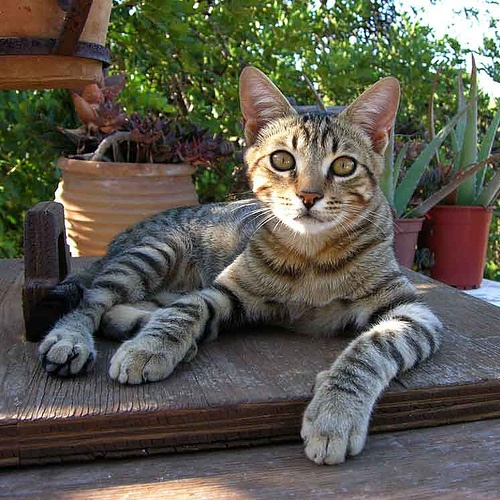
\includegraphics[width=0.20\textwidth,height=0.20\textwidth]{figures/originals/2007_003778}
%       & 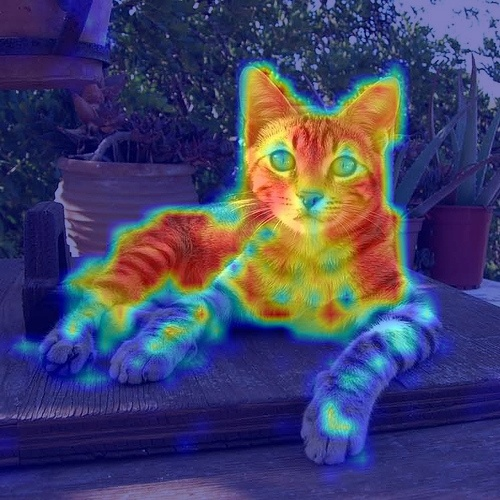
\includegraphics[width=0.20\textwidth,height=0.20\textwidth]{figures/val_cams/weclip/2007_003778_7}
%       & 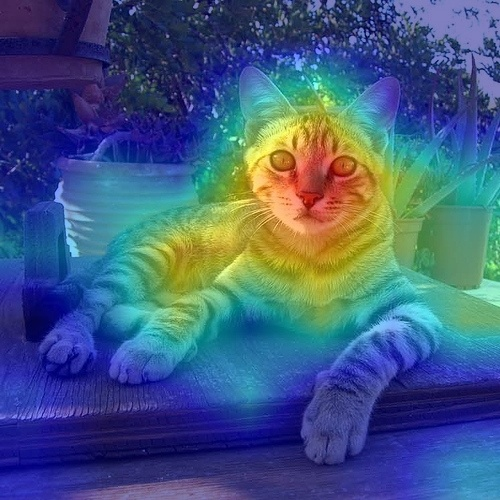
\includegraphics[width=0.20\textwidth,height=0.20\textwidth]{figures/val_cams/ours/2007_003778_7}
%       \\

%       \textbf{Bicycle}
%       & 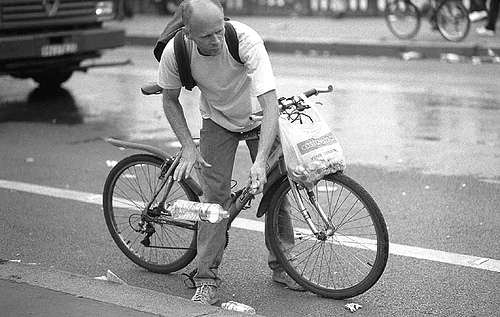
\includegraphics[width=0.20\textwidth,height=0.20\textwidth]{figures/originals/2011_000453}
%       & 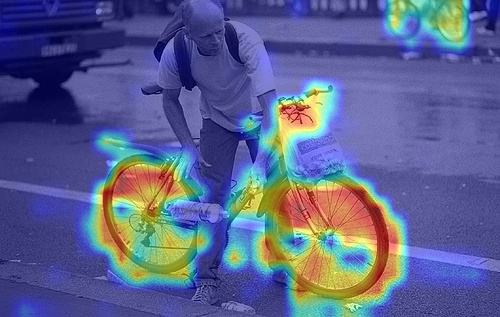
\includegraphics[width=0.20\textwidth,height=0.20\textwidth]{figures/val_cams/weclip/2011_000453_1}
%       & 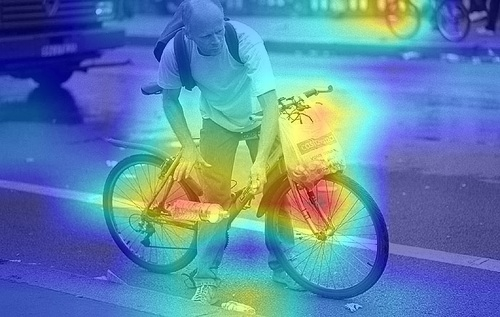
\includegraphics[width=0.20\textwidth,height=0.20\textwidth]{figures/val_cams/ours/2011_000453_1}
%       \\

%       \textbf{Bird}
%       & 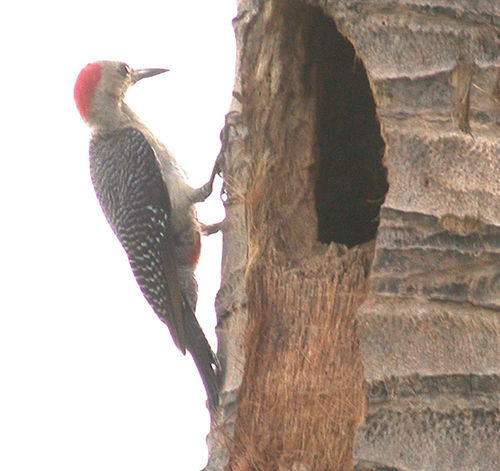
\includegraphics[width=0.20\textwidth,height=0.20\textwidth]{figures/originals/2011_001902}
%       & 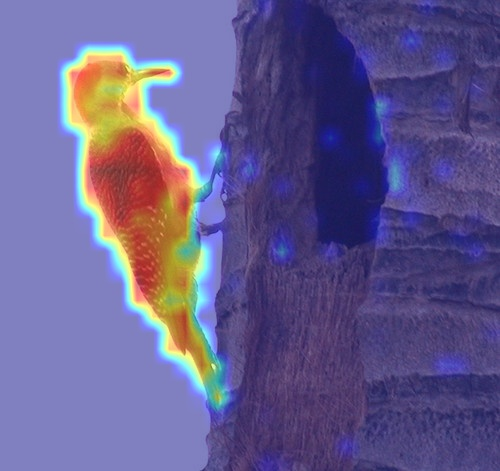
\includegraphics[width=0.20\textwidth,height=0.20\textwidth]{figures/val_cams/weclip/2011_001902_2}
%       & 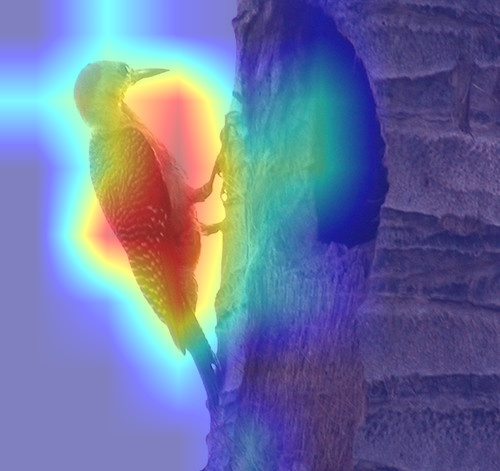
\includegraphics[width=0.20\textwidth,height=0.20\textwidth]{figures/val_cams/ours/2011_001902_2}
%       \\

%       \textbf{Boat}
%       & 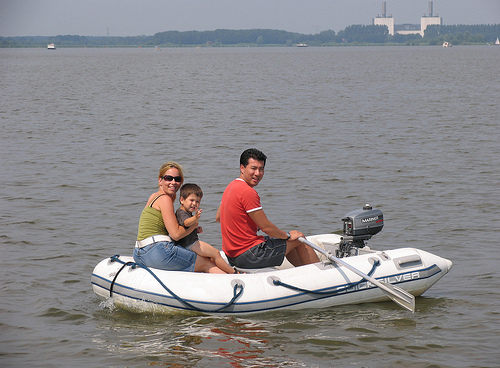
\includegraphics[width=0.20\textwidth,height=0.20\textwidth]{figures/originals/2010_003599}
%       & 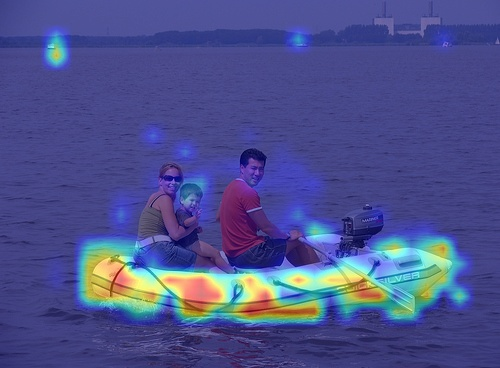
\includegraphics[width=0.20\textwidth,height=0.20\textwidth]{figures/val_cams/weclip/2010_003599_3}
%       & 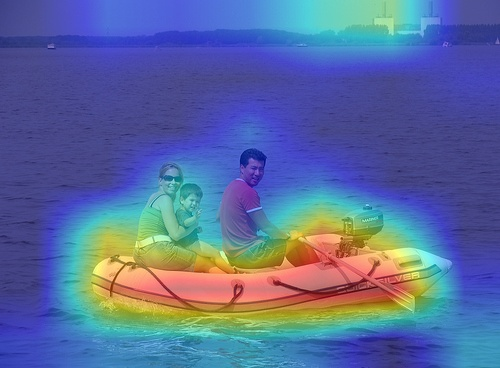
\includegraphics[width=0.20\textwidth,height=0.20\textwidth]{figures/val_cams/ours/2010_003599_3}
%     \end{tabular}
%   \end{tcolorbox}

%   \caption{Qualitative comparison of CAMs between WeCLIP and our UniCL-AffSeg on PASCAL VOC 2012 \textit{val} set (first 4 classes).}
%   \label{fig:qualitative_comparison_cam_val_1}
% \end{figure}

% \begin{figure}[ht]
%   \centering
%   \setlength{\tabcolsep}{2pt}
%   \renewcommand{\arraystretch}{0.9}

%   \begin{tcolorbox}[colframe=black!60, colback=white, boxrule=0.8pt, arc=2pt, left=2pt, right=2pt, top=2pt, bottom=2pt]
%     \centering
%     \begin{tabular}{m{3cm} c c c}

%       & (a) Input & (b) WeCLIP & (c) Ours
%       \\ [1mm]

%       \textbf{Pottedplant}
%       & 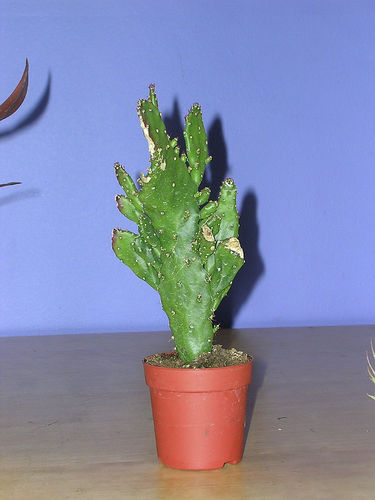
\includegraphics[width=0.20\textwidth,height=0.20\textwidth]{figures/originals/2011_000145}
%       & 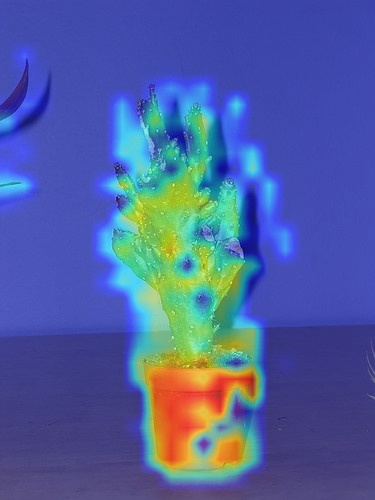
\includegraphics[width=0.20\textwidth,height=0.20\textwidth]{figures/val_cams/weclip/2011_000145_15}
%       & 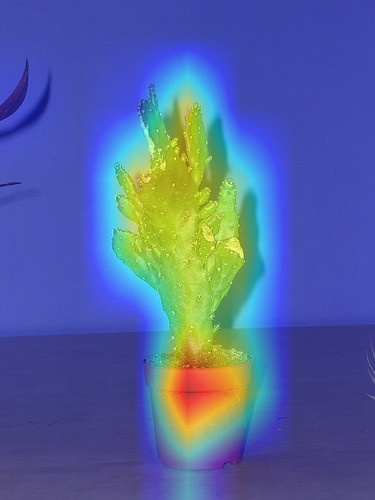
\includegraphics[width=0.20\textwidth,height=0.20\textwidth]{figures/val_cams/ours/2011_000145_15}
%       \\

%       \textbf{Car}
%       & 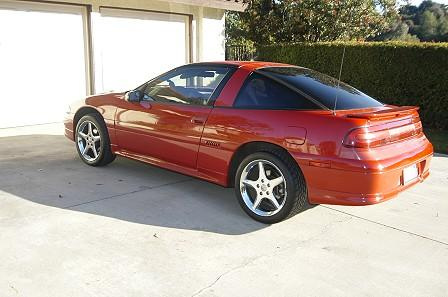
\includegraphics[width=0.20\textwidth,height=0.20\textwidth]{figures/originals/2010_005119}
%       & 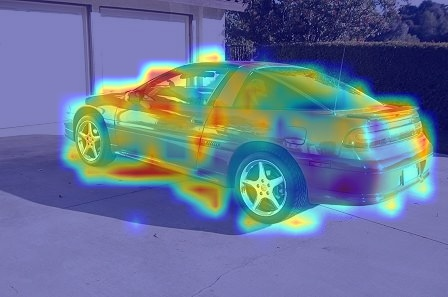
\includegraphics[width=0.20\textwidth,height=0.20\textwidth]{figures/val_cams/weclip/2010_005119_6}
%       & 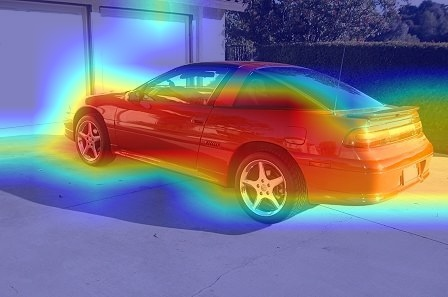
\includegraphics[width=0.20\textwidth,height=0.20\textwidth]{figures/val_cams/ours/2010_005119_6}
%       \\

%       \textbf{Bus}
%       & 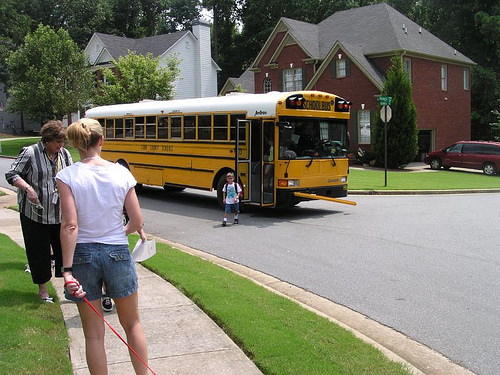
\includegraphics[width=0.20\textwidth,height=0.20\textwidth]{figures/originals/2010_000148}
%       & 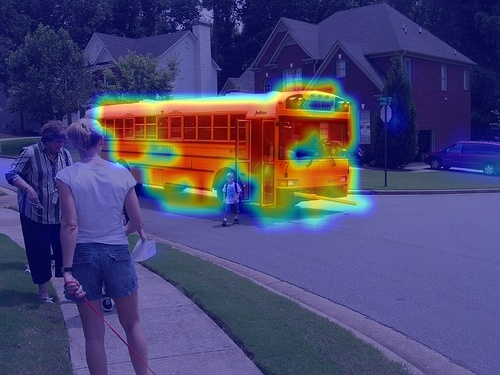
\includegraphics[width=0.20\textwidth,height=0.20\textwidth]{figures/val_cams/weclip/2010_000148_5}
%       & 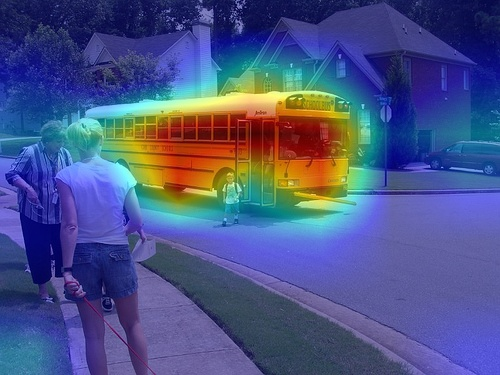
\includegraphics[width=0.20\textwidth,height=0.20\textwidth]{figures/val_cams/ours/2010_000148_5}
%       \\

%       \textbf{Person}
%       & 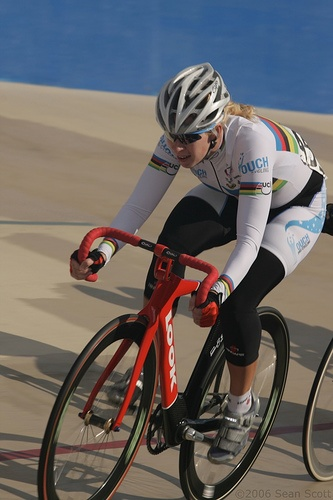
\includegraphics[width=0.20\textwidth,height=0.20\textwidth]{figures/originals/2007_005702}
%       & 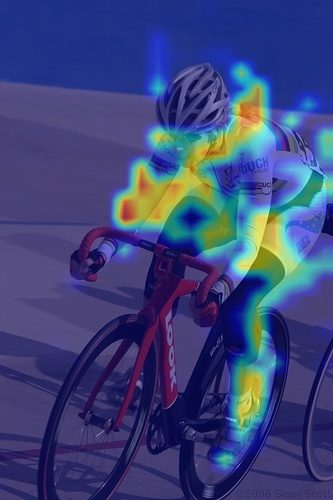
\includegraphics[width=0.20\textwidth,height=0.20\textwidth]{figures/val_cams/weclip/2007_005702_14}
%       & 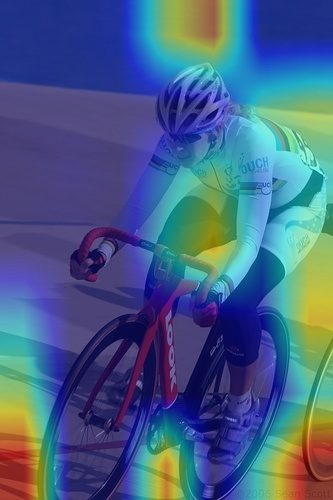
\includegraphics[width=0.20\textwidth,height=0.20\textwidth]{figures/val_cams/ours/2007_005702_14}
%     \end{tabular}
%   \end{tcolorbox}

%   \caption{Qualitative comparison of CAMs between WeCLIP and our UniCL-AffSeg on PASCAL VOC 2012 \textit{val} set (last 4 classes).}
%   \label{fig:qualitative_comparison_cam_val_2}
% \end{figure}


